\documentclass[12pt,openany]{report}      % paper size is in preamble.sty

%\usepackage[utf8x]{inputenc}
%\renewcommand*\sfdefault{ugq}
\usepackage[T1]{fontenc}
\usepackage{lmodern}
\usepackage{graphicx}
\usepackage{booktabs}
%\usepackage[a4paper]{geometry}
\usepackage[top=1in, bottom=1.25in, left=0.5in, right=0.5in]{geometry}

\def\TITLE{NORDAN 26}
\def\SUBTITLE{Nordic Complex Analysis Meeting}
\def\LOCATION{Hella, Iceland -- May 23-25, 2025}

\begin{document}
\begin{titlepage}
	\centering
	%\vpspace{3cm}
    {\textbf{\textsf{\fontsize{63}{18}\selectfont \TITLE}}\par}
	\vspace{0.5cm}
	{\Huge \textsf{\SUBTITLE}\par}
	\vspace{0.5cm}
	{\Large \LOCATION\par}
	\vspace{2cm}
	\vfill
    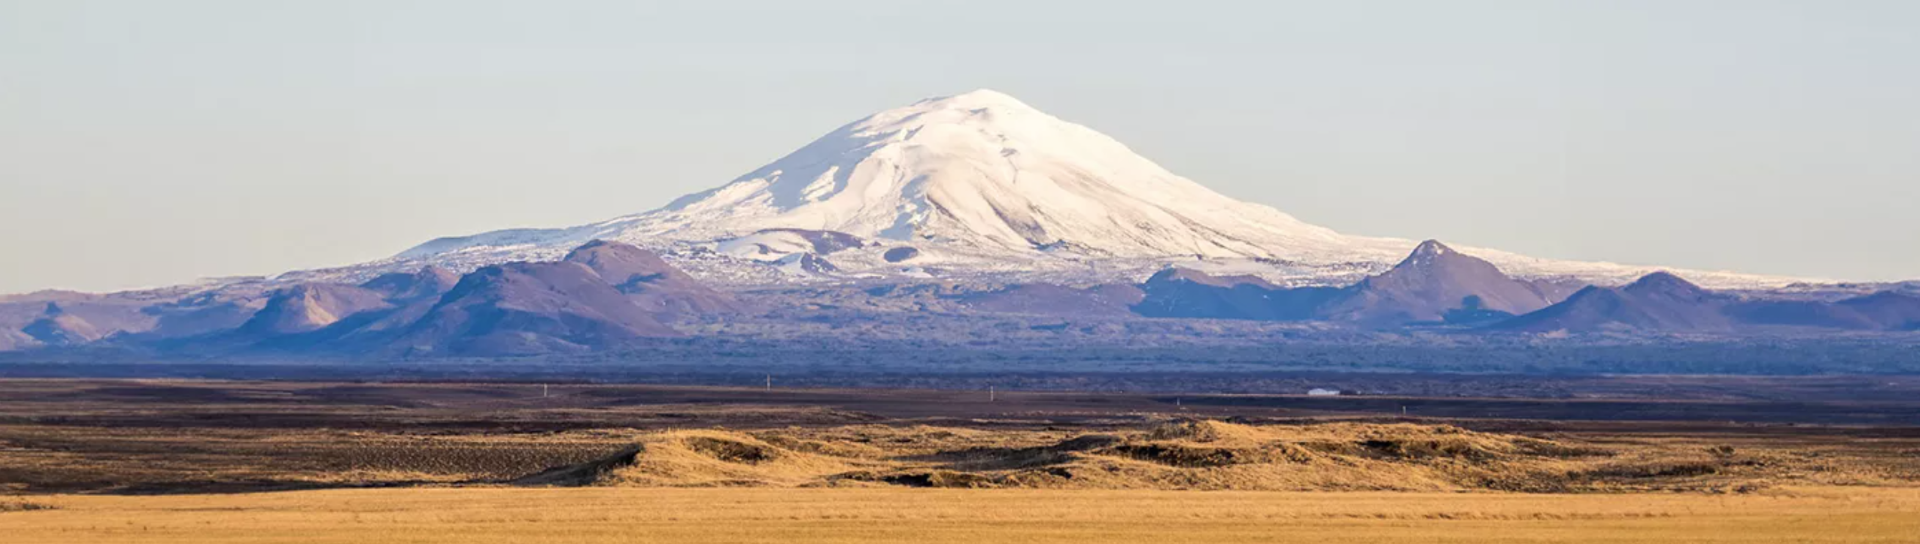
\includegraphics[width=1\textwidth]{cover}\par\vspace{1cm}
\end{titlepage}

\newpage
\begin{center} 
    \noindent\fbox{\begin{minipage}{0.7\textwidth}
        \centering Nice text in a box
    \end{minipage}}
\end{center}
    
\vfill

Organizers:
\begin{itemize}
    \item Benedikt Steinar Magnússon, University of Iceland
    \item Álfheiður Edda Sigurðardóttir, IMFM, Ljubljana
    \item Bergur Snorrason, University of Iceland
    \item Gianmarco Brocchi, University of Iceland
\end{itemize}



\newpage

\begin{tabular}{llll}
    \toprule
    \multicolumn{4}{c}{Nordan - Nordic Complex Analysis Meeting}\\
    \midrule
     & Year & Location & Organizers \\
     \midrule
    1 & 1997 & Trosa & Stockholm University  \\
    2 & 1998 & Marstrand & Chalmers University of Technology/\\
      &      &               & University of Gothenburg \\
    3 & 1999 & Saltsjöbaden & Stockholm University  \\
    4 & 2000 & Örnköldsvik & Mid Sweden University/Umeå University\\
    5 & 2001 & Voksenåsen & University of Oslo \\
    6 & 2002 & Reykjavik & University of Iceland \\
    7 & 2003 & Visby & Stockholm University\\
    8 & 2004 & Nösund, Orust & Chalmers University of Technology/\\
       &      &               & University of Gothenburg \\
    9 & 2005 & Sigtuna & Uppsala University \\
    10 & 2006 & Sundsvall & Mid Sweden University/Umeå University \\
    11 & 2007 & Drøbak & University of Oslo\\
    12 & 2008 & Mariehamn, Åland & Stockholm University - Part of the Mittag-Leffler program\\
    13 & 2009 & 
    Reykholt & University of Iceland\\
    14 & 2010 & Lökeberg & Chalmers University of Technology/\\
       &      &               & University of Gothenburg\\
    15 & 2011 & Röstånga & Lund University\\
    16 & 2012 & Kiruna & Mid Sweden University/Umeå University\\
    17 & 2013 & Svolvær & University of Oslo\\
    18 & 2014 & Luminy & CIRM - Nordan+Kawa\\
    19 & 2015 & Reykjavik & University of Iceland\\
    20 & 2016 & Stockholm & Part of the 27th Nordic Congress of Mathematics\\
    21 & 2017 & Tollered & Chalmers University of Technology/\\
       &      &               & University of Gothenburg\\
    22 & 2018 & Hjelmeland & University of Stavanger\\
    23 & 2019 & Lunteren & University of Amsterdam\\
    24 & 2023 & Rydebäck & Lund University\\
    25 & 2024 & Östanskär & Mid Sweden University/Umeå University\\
    26 & 2025 & Hella & University of Iceland\\
%    27 & 2026 & TBA & University of Eastern Finland & NaN & NaN & NaN & NaN & NaN \\
    \bottomrule
    \end{tabular}
    
\begin{tabular}{llll}
        \toprule
        \multicolumn{4}{c}{KAUS - Complex Analysis without Seniors}\\
        \midrule
         & Year & Location & Organizers \\
         \midrule
        1 & 2005 & Umeå & Umeå University\\
        2 & 2006 & Göteborg  & Chalmers University of Technology/\\
          &      &               & University of Gothenburg \\
        3 & 2007 & Sundsvall & Mid Sweden University\\
        4 & 2007 & Stockholm & Stockholm University  \\
        5 & 2009 & Reykjavík & University of Iceland\\
        6 & 2010 & Umeå & Umeå University\\
        7 & 2010 & Göteborg & Chalmers University of Technology/\\
           &      &               & University of Gothenburg\\
        8 & 2024 & Östanskär & Mid Sweden University/Umeå University\\
        9 & 2025 & Reykjavík & University of Iceland\\
    %    27 & 2026 & TBA & University of Eastern Finland & NaN & NaN & NaN & NaN & NaN \\
        \bottomrule
        \end{tabular}
\end{document}


\documentclass[A4paper,openany]{book}
\usepackage[pdftex]{graphicx}
\usepackage{amsmath}
\usepackage{amssymb}
\usepackage{tipa}
%\usepackage{txfonts}
\usepackage{textcomp}
%\usepackage{amsthm}
%\usepackage{array}
%\usepackage{xy}
\usepackage{fancyhdr}
